%%%%%%%%%%%%%%%%%%%%%%%%%%%%%%%%%%%%%%%%%%%%%%%%%%%%%%%%%%%%%%%%%%%%%%%%%%%%%%
% A Self-Learning Utility-Based Agent for Adaptive Data-Pipeline Orchestration:
% An Environment-Optimiser-Reward Taxonomy of the Always-Execute Attractor.
% Single-author, independent version.
%%%%%%%%%%%%%%%%%%%%%%%%%%%%%%%%%%%%%%%%%%%%%%%%%%%%%%%%%%%%%%%%%%%%%%%%%%%%%%

\documentclass[10pt,twocolumn]{article}

% ---- Encoding, layout, typography -------------------------------------------
\usepackage[utf8]{inputenc}
\usepackage[T1]{fontenc}
\usepackage[a4paper,margin=1in,headheight=15pt]{geometry}
\usepackage{lmodern}
\usepackage{microtype}
\usepackage{setspace}
\setstretch{1.02}
\setlength{\columnsep}{0.24in}
\setlength{\emergencystretch}{3em}
\clubpenalty=10000
\widowpenalty=10000
\displaywidowpenalty=10000

% ---- Colour, boxes ----------------------------------------------------------
\usepackage{xcolor}
\definecolor{accent}{RGB}{0,0,128}
\usepackage[most]{tcolorbox}

% ---- Graphics, floats, captions ---------------------------------------------
\usepackage{graphicx}
\usepackage{float}
\usepackage{dblfloatfix}
\usepackage[font=small,labelfont=bf]{caption}
\usepackage{subcaption}
\captionsetup{skip=4pt}

% ---- Maths, algorithms, code ------------------------------------------------
\usepackage{amsmath,amssymb,amsthm,mathtools}
\allowdisplaybreaks
\usepackage{algorithm}
\usepackage{algpseudocode}
\usepackage{listings}
\lstset{basicstyle=\footnotesize\ttfamily,breaklines=true,
  breakatwhitespace=true,columns=fullflexible,keepspaces=true,
  showstringspaces=false,frame=single}

% ---- Tables, lists ----------------------------------------------------------
\usepackage{booktabs,tabularx,array,makecell,adjustbox,multirow}
\usepackage[shortlabels]{enumitem}
\renewcommand{\arraystretch}{1.15}
\setlist[itemize]{leftmargin=1.2em,itemsep=2pt,topsep=3pt}
\setlist[enumerate]{leftmargin=1.4em,itemsep=2pt,topsep=3pt}
\newcolumntype{Y}{>{\raggedright\arraybackslash}X}
\newcolumntype{C}{>{\centering\arraybackslash}X}

% ---- Hyperlinks -------------------------------------------------------------
\usepackage{xurl}
\usepackage{csquotes}
\usepackage[colorlinks=true,linkcolor=black,citecolor=black,
  urlcolor=blue!50!black]{hyperref}
\urlstyle{same}

% ---- Header / footer --------------------------------------------------------
\usepackage{fancyhdr}
\pagestyle{fancy}
\fancyhf{}
\fancyhead[L]{\small An Environment--Optimiser--Reward Taxonomy of the Always-Execute Attractor}
\fancyhead[R]{\small \thepage}
\renewcommand{\headrulewidth}{0.4pt}
\fancypagestyle{plain}{\fancyhf{}\fancyhead[R]{\small \thepage}\renewcommand{\headrulewidth}{0pt}}

% ---- Section formatting -----------------------------------------------------
\usepackage{titlesec}
\titleformat{\section}{\normalfont\Large\bfseries}{\thesection.}{0.6em}{}
\titleformat{\subsection}{\normalfont\large\bfseries}{\thesubsection.}{0.6em}{}
\titleformat{\subsubsection}{\normalfont\normalsize\bfseries}{\thesubsubsection.}{0.6em}{}
\titlespacing*{\section}{0pt}{10pt plus 2pt minus 2pt}{5pt}
\titlespacing*{\subsection}{0pt}{8pt plus 2pt minus 2pt}{4pt}
\titlespacing*{\subsubsection}{0pt}{6pt plus 2pt minus 2pt}{3pt}

% ---- Bibliography -----------------------------------------------------------
\usepackage[backend=biber,style=ieee]{biblatex}
\addbibresource{references.bib}

% ---- Macros -----------------------------------------------------------------
\newcommand{\agent}[1]{\textsc{#1}}
\newcommand{\term}[1]{\texttt{#1}}
\newcommand{\env}[1]{\texttt{#1}}

%%%%%%%%%%%%%%%%%%%%%%%%%%%%%%%%%%%%%%%%%%%%%%%%%%%%%%%%%%%%%%%%%%%%%%%%%%%%%%
\begin{document}

% ---- Title block ------------------------------------------------------------
\twocolumn[
  \begin{center}
    {\fontsize{17pt}{21pt}\selectfont\bfseries
      A Self-Learning Utility-Based Agent for Adaptive\\
      Data-Pipeline Orchestration: An Environment--Optimiser--Reward\\
      Taxonomy of the Always-Execute Attractor\par}
    \vspace{0.7em}
    {\large Ahmed Mamdouh Mohamed Mohamed\par}
    \vspace{0.2em}
    {\normalsize Independent Researcher\quad\textbar\quad
      \href{mailto:ahmdmshazly@gmail.com}{ahmdmshazly@gmail.com}\par}
    \vspace{0.5em}
    \textcolor{accent}{\rule{0.85\textwidth}{0.8pt}}
    \vspace{0.6em}
  \end{center}
]

% ---- Abstract ---------------------------------------------------------------
\begin{abstract}
\noindent
Adaptive data-pipeline orchestration in cloud environments requires balancing
pipeline value, compute cost, and failure risk under uncertainty. A natural
design is a self-learning agent that maximises a single scalar utility
$U=\alpha\,\mathrm{Value}-\beta\,\mathrm{Cost}-\gamma\,\mathrm{Risk}$. On a
discrete-action simulator with one hundred jobs per episode, such an agent
trained with policy gradient converges to a deterministic \emph{always-execute}
policy --- it launches a ready task at every step and never scales, defers, or
pauses. The tempting conclusion, drawn in an earlier version of this work, is
that the \emph{shape} of the scalar reward determines this trivial attractor.
This paper shows that conclusion is wrong, and replaces it with a measured
taxonomy. We hold the reward family fixed and vary, one at a time, the three
factors a scalar-utility scheduler actually depends on: the environment, the
optimiser, and the reward specification. Across five environments and two
policy-gradient algorithms (REINFORCE and PPO), each with three initialisation
seeds and fifty held-out evaluation seeds, always-execute appears for three
\emph{distinct} reasons. (i) On a benign environment, always-execute is the
genuine optimum of the true objective --- a Monte-Carlo policy-improvement probe
shows no single non-execute deviation has positive advantage --- so the learner
is correct, not pathological. (ii) On environments where a non-execute action
provably pays (contended capacity; load-dependent failure; heavy-tailed value),
REINFORCE remains stuck at always-execute, but PPO escapes and beats it by
$+14$ to $+28$ utility units ($p<10^{-5}$), so the attractor is a property of the
\emph{weak optimiser}, not the reward. (iii) A defect in the original per-step
reward --- its risk term telescopes to a decaying counter rather than to the
failed-job count, so the cumulative reward does not equal the reported utility
--- suppresses caution; correcting it changes a reckless policy (51\% failure
rate) into a careful one (5\%). We further show, with an adequately powered test
($n{=}250$), that the learned policy is significantly, if slightly, worse than a
trivial reflex baseline ($-3.06$ utility, $p=2.3\times10^{-3}$), correcting an
earlier underpowered claim of equivalence ($p=0.08$ at $n{=}50$, $28.8\%$ power).
The contribution is a reproducible diagnosis: a scalar-utility scheduler that
``looks trivial'' is explained by its environment, its optimiser, or a
reward-specification bug --- and a competent learner adapts, scaling where
scaling pays, throttling where caution pays, and abstaining where neither does.
\end{abstract}

\vspace{0.4em}
{\small\noindent\textbf{Keywords:} reinforcement learning, data-pipeline
orchestration, reward design, negative results, proximal policy optimization,
reproducibility.}
\vspace{0.6em}

% =============================================================================
\section{Introduction}
\label{sec:intro}

Modern data pipelines run in cloud environments where workload intensity,
resource availability, spot-price, and execution failures vary over time. In
such settings, orchestration decisions cannot be reduced to static scheduling
rules, because the same action can have very different consequences depending on
congestion, price, contention, and recent failures. This makes adaptive pipeline
orchestration a sequential decision problem rather than only a
workflow-engineering one.

A practitioner reaching for a learned solution will naturally encode the
competing objectives --- complete valuable work, control compute cost, avoid
unstable or failure-prone decisions --- as a single scalar utility
\begin{equation}
\label{eq:utility}
U \;=\; \alpha\cdot\mathrm{Value}\;-\;\beta\cdot\mathrm{Cost}\;-\;\gamma\cdot\mathrm{Risk},
\end{equation}
and train an agent to maximise it. This paper studies what such an agent learns,
and why.

On a discrete-action, single-cluster orchestration simulator with one hundred
jobs per episode and realistic stochastic events, an agent trained by policy
gradient on Eq.~\eqref{eq:utility} converges to a deterministic
\emph{always-execute} policy: at every decision step it launches a ready task,
and it never scales the cluster, defers, reprioritises, or pauses. Five of its
six actions receive near-zero probability. The same outcome survives an
eighty-one-cell sweep of $(\alpha,\beta,\gamma)$, an expansion of the observation
from eight to fourteen dimensions, and three network-initialisation seeds.

An earlier version of this work concluded from these invariances that the
\emph{shape} of the committed reward --- not the algorithm and not the
observation --- determines the always-execute attractor, and framed it as a
reward-shape-induced ``trivial-attractor failure mode.'' The present paper
reports a skeptical re-examination of that claim and finds it does not hold. The
earlier experiments varied three factors (reward weights, observation, seed) but
held fixed the one factor that actually controls whether any non-execute action
has positive expected value: the \emph{environment}. They also rested on a
per-step reward whose cumulative value does not equal the reported episode
utility, and on an equivalence claim made at a sample size with $28.8\%$
statistical power.

\paragraph{Contributions.} We replace the single-cause claim with a measured,
reproducible taxonomy.
\begin{enumerate}
\item \textbf{A reward-specification defect (\S\ref{sec:reward-bug}).} The
per-step reward used to train the agent telescopes, on its risk term, to a
decaying failure counter rather than to the failed-job count used by the
evaluation metric. Hence the cumulative reward is \emph{not} the episode utility:
the learner trains with an effectively zero failure penalty. We provide a
config-gated correction for which the cumulative reward equals the utility
exactly, verified by test.
\item \textbf{The benign environment has a trivial optimum
(\S\ref{sec:benign}).} A common-random-number Monte-Carlo policy-improvement
probe shows that on the committed environment no single non-execute deviation
from always-execute has a positive-advantage confidence interval. Always-execute
is the true optimum; the learner is correct.
\item \textbf{An adequately powered comparison (\S\ref{sec:power}).} On a
pre-registered, disjoint evaluation pool of $250$ seeds, the learned policy is
significantly --- though slightly --- \emph{worse} than a trivial reflex
baseline ($-3.06$ utility, $p=2.3\times10^{-3}$), overturning an earlier
underpowered claim of equivalence.
\item \textbf{The attractor is optimiser-determined, not reward-determined
(\S\ref{sec:taxonomy}).} On three environments engineered so that a non-execute
action provably pays, REINFORCE remains at always-execute on $6/6$
scaling-lever seeds, whereas PPO escapes on $5/6$ and beats always-execute by
$+14$ to $+28$ utility units ($p<10^{-5}$). Under the identical reward and
environment, a stronger optimiser removes the attractor. PPO also \emph{abstains}
correctly: on the benign environment it stays at always-execute.
\item \textbf{The reward defect is material (\S\ref{sec:taxonomy}).} On an
environment where overload causes cascading failures, the original (buggy)
reward leaves even PPO largely reckless ($51\%\!\to\!44\%$ failure), while the
corrected reward turns REINFORCE into a careful policy ($51\%\!\to\!5\%$ failure,
$+120$ utility).
\end{enumerate}

The honest synthesis (\S\ref{sec:discussion}) is that a scalar-utility scheduler
which ``looks trivial'' is explained by the environment (the optimum really is
trivial), the optimiser (a real but modest improvement the algorithm cannot
find), or a reward-specification bug --- never by ``reward shape'' as a
standalone cause. We position this against four literatures
(\S\ref{sec:related}) and discuss why the constrained-MDP reformulation an
earlier draft proposed as ``the corrective'' is mistargeted
(\S\ref{sec:discussion}).

% =============================================================================
\section{Related Work}
\label{sec:related}

This paper sits at the intersection of four literatures: learned schedulers for
cloud and cluster systems, negative results and simple-baseline equivalence in
deep reinforcement learning, reward design and reward hacking, and constrained
Markov decision processes.

\subsection{Learned Scheduling and Resource Management}
The use of reinforcement learning for cluster and pipeline scheduling begins with
DeepRM \cite{mao2016deeprm}, which casts multi-resource packing as a
policy-gradient problem and trains a REINFORCE agent against a negative-sojourn
reward. Decima \cite{mao2019decima} extends the formulation to DAG-structured
Spark workloads, coupling a graph-neural-network encoder over the ready frontier
with an actor--critic policy and an input-dependent baseline \cite{mao2019variance},
reducing average job completion time on TPC-H workloads. Non-RL approaches cover
the same design space with other machinery: CherryPick \cite{alipourfard2017cherrypick}
performs Bayesian optimisation over VM configurations under a runtime SLO;
Resource Central \cite{cortez2017resource} trains supervised predictors for
downstream schedulers. A market- and optimisation-theoretic line expresses
allocation as constrained convex or game-theoretic problems: Gavel
\cite{narayanan2020gavel} re-expresses scheduling policies as linear programs
over an effective-throughput matrix; Pollux \cite{qiao2021pollux} maximises a
concave goodput metric; Sia \cite{subramanya2023sia} and Shockwave
\cite{zheng2023shockwave} extend goodput to heterogeneous clusters and to
dynamic-adaptation market equilibria. The contemporary LLM-serving lineage ---
vLLM \cite{kwon2023vllm}, Sarathi-Serve \cite{agrawal2024sarathi}, DistServe
\cite{zhong2024distserve} --- optimises SLO-constrained goodput under hard
latency and memory budgets.

The divergence between our setting and this lineage is the \emph{reward shape}.
Each of DeepRM, Decima, Pollux, and the LLM-serving schedulers optimises an
objective whose optimum is structurally non-trivial --- through backpressure, an
integrated completion-time penalty under stochastic arrivals, concavity, or hard
constraints --- so that ``admit every ready job immediately'' is not a local
optimum. Our scalarised utility~\eqref{eq:utility} lacks any analogous structural
non-triviality. The present paper investigates exactly when that absence makes
the optimum trivial, and finds that it is an environment property, not a property
of the linear form.

\subsection{Negative Results and Simple-Baseline Equivalence}
A smaller, less-visible literature documents, rather than circumvents,
reinforcement learning's failure to beat simple baselines. Mania, Guy, and Recht
\cite{mania2018ars} show that augmented random search over linear policies
matches state-of-the-art deep RL on MuJoCo; Rajeswaran et al.
\cite{rajeswaran2017simplicity} show the same for linear and RBF policies.
Henderson et al. \cite{henderson2018matters} and Engstrom et al.
\cite{engstrom2020implementation} document the reproducibility and
implementation-attribution problems that make point-estimate comparisons
unreliable; Andrychowicz et al. \cite{andrychowicz2021what} find low-level design
choices dominate algorithmic identity. Agarwal et al. \cite{agarwal2021precipice}
and Jordan et al. \cite{jordan2020evaluating} supply the statistical machinery
--- stratified bootstrap, interquartile mean, probability of improvement,
performance profiles --- that makes null results visible rather than hidden
behind a mean. We adopt that machinery directly (\S\ref{sec:power}), and we
emphasise the lesson it implies but that the present setting makes vivid: an
apparent equivalence to a simple baseline can be an artifact of low statistical
power, and a deep-RL ``failure'' can be a property of the optimiser rather than
of the objective.

\subsection{Reward Design and the Shape of the Objective}
Ng, Harada, and Russell's potential-based shaping theorem \cite{ng1999shaping}
establishes that adding a potential-difference term to a reward preserves the set
of optimal policies. This is frequently glossed as ``the shape of a reward
determines the optimal policy set,'' but the theorem concerns \emph{additive
potential-based shaping}, not the question of whether a given linear
scalarisation of competing objectives has a trivial optimum on a given MDP; it
therefore motivates, rather than entails, the present study. Amodei et al.
\cite{amodei2016concrete} frame reward misspecification as a non-adversarial
failure mode. Skalse et al. \cite{skalse2022hacking} define and characterise
reward hacking and the conditions under which a reward simplification is
``unhackable''; this constrains when a coarsening preserves a policy ordering but
does not imply that linear scalarisations generically collapse to a dominating
simplification. Pan et al. \cite{pan2022misspecification} give empirical evidence
that reward ``misweighting'' produces phase transitions to degenerate behaviour;
Knox et al. \cite{knox2023reward} provide sanity checks for reward design. The
multi-objective RL literature \cite{roijers2013morl,vamplew2022scalar} argues
that scalar reward is structurally insufficient for multi-attribute tasks and
formalises Pareto and convex coverage sets as alternatives. The present paper is
a minimally confounded case study within this body: we show that the apparent
triviality is governed by the environment and the optimiser, isolate a concrete
reward-specification bug, and decline to attribute the outcome to ``reward
shape'' once those factors are varied.

\subsection{Constrained MDPs as a Proposed Reformulation}
A fixed linear scalarisation is the Lagrangian of a constrained MDP
\cite{altman1999cmdp} at fixed dual multipliers: maximising
$\mathbb{E}[V]$ subject to $\mathbb{E}[C]\le c_{\max}$ and
$\mathbb{E}[R]\le r_{\max}$ has Lagrangian $\mathbb{E}[V]-\lambda_C\mathbb{E}[C]-
\lambda_R\mathbb{E}[R]$, which at fixed $\lambda$ is exactly
Eq.~\eqref{eq:utility}. Reward-Constrained Policy Optimisation
\cite{tessler2019rcpo}, the PID-Lagrangian method \cite{stooke2020pid},
Constrained Policy Optimisation \cite{achiam2017cpo}, Lyapunov-based safe RL
\cite{chow2018lyapunov}, and projection- and interior-point alternatives
\cite{yang2020pcpo,liu2020ipo} learn the multipliers instead of fixing them.
An earlier draft proposed this reformulation as ``the corrective'' for the
trivial attractor. We revisit that proposal in \S\ref{sec:discussion} and argue
it is mistargeted: a CMDP cannot create a non-trivial optimum where the
environment has none, and where the environment does provide a lever, a stronger
optimiser or the corrected scalar reward already suffices.

% =============================================================================
\section{The Orchestration Environment}
\label{sec:env}

The evaluation environment is a discrete-time, single-cluster simulator of a
stochastic data-pipeline orchestration setting. An episode is a sequence of
decision steps; at each step the agent observes a normalised state vector,
selects one of six actions, and the world advances one tick. Every numeric
parameter is read from a single configuration file; no constant is hard-coded in
the agent or environment source. The simulator is deterministic given a seed:
each seed spawns two independent \texttt{numpy} generators (one for the workload,
one for the stochastic events) so that workload and event traces are reproducible
independently.

\subsection{State, Actions, Cost}
\label{sec:state-actions}

\paragraph{State.} The observation is a vector of eight real-valued features in
$[0,1]$ (Table~\ref{tab:state}); a fourteen-dimensional richer variant appends
five per-job queue features and one spot-price forecast, used only where noted.

\paragraph{Actions.} At each step the agent selects one of six named actions with
fixed parameters (Table~\ref{tab:actions}). Every action is legal from every
reachable state; actions with no applicable target behave as no-ops.

\paragraph{Cost.} The per-step cost is
$\mathrm{cost}(s,a)=p_{\mathrm{spot}}(s)\,(w_{\mathrm{cpu}}\,\mathrm{cpu}_{\mathrm{in\,use}}+w_{\mathrm{ram}}\,\mathrm{ram}_{\mathrm{in\,use}})$
with $w_{\mathrm{cpu}}=0.6$, $w_{\mathrm{ram}}=0.4$, plus a per-action tariff that
is zero in the committed configuration. Episode cost is the sum over steps.

\begin{table}[t]
\centering
\caption{State vector $S\in[0,1]^8$ (committed observation). A fourteen-dimensional
variant appends five queue features and one spot-price forecast.}
\label{tab:state}
\small
\begin{tabularx}{\columnwidth}{@{}lY@{}}
\toprule
\textbf{Feature} & \textbf{Meaning} \\
\midrule
$\ell_{\mathrm{cpu}}$        & CPU load (in-use / capacity) \\
$r_{\mathrm{ram}}$           & free-RAM fraction \\
$q$                          & ready-queue depth (saturated at 20) \\
$p_{\mathrm{spot}}$          & current spot price, $[0.1,1.0]$ \\
$n_{\mathrm{ready}}$         & DAG-ready nodes (saturated at 20) \\
$p_{\mathrm{job}}$           & mean priority over active jobs \\
$u_{\mathrm{deadline}}$      & mean deadline urgency over active jobs \\
$f_{\mathrm{recent}}$        & recent-failure counter (saturated at 5) \\
\bottomrule
\end{tabularx}
\end{table}

\begin{table}[t]
\centering
\caption{Action space. Parameters are fixed across a run.}
\label{tab:actions}
\small
\begin{tabularx}{\columnwidth}{@{}lY@{}}
\toprule
\textbf{Action} & \textbf{Effect} \\
\midrule
\term{Execute\_Ready\_Job}   & launch the ready task maximising $\mathrm{value}\times\mathrm{priority}$ if it fits; else no-op \\
\term{Defer\_Job}            & one-step no-op; time advances \\
\term{Scale\_Up}             & $+3$ CPU, $+4$ RAM for three steps, then decays \\
\term{Scale\_Down}           & $-2$ CPU, $-2$ RAM, floored at the cluster minimum \\
\term{Reprioritize\_Queue}   & $+0.05$ priority to every queued job (cap $1.0$) \\
\term{Pause\_LowPriority\_Job} & pause up to two running low-priority jobs \\
\bottomrule
\end{tabularx}
\end{table}

\subsection{Stochastic Processes and the Workload}
\label{sec:stochastic}
Three exogenous processes drive non-determinism: a node-failure process, a
data-spike process, and a bounded random walk on the spot price. Each has an
explicit \texttt{mode} so that alternatives can be selected without code changes;
this is the mechanism by which we vary the environment in
\S\ref{sec:taxonomy}. Each episode instantiates $N=100$ jobs by cloning one of
three DAG templates (a linear chain, a fork--join, and a three-source
aggregation) and perturbing durations and resource demands by discrete factors.
Per-job value is drawn from $U(1,5)$ in the committed (benign) workload; a
heavy-tailed variant (\S\ref{sec:env-family}) replaces a fraction of jobs with
high-value ``whales.''

\subsection{The Shared Utility and Its Three Roles}
\label{sec:utility}
The episode utility is
\begin{equation}
\label{eq:episode-utility}
U \;=\; \alpha\!\sum_{\text{completed}}\!\mathrm{Value}
   \;-\; \beta\,\mathrm{TotalCost}
   \;-\; \gamma\,|\text{FailedJobs}|,
\end{equation}
with committed weights $(\alpha,\beta,\gamma)=(1.0,0.1,1.0)$. The same scalar is
intended to play three roles: the evaluation metric, the scoring term of the
non-learning Utility-Based agent, and the reward signal for the learner. This
``three-role identification'' is the methodological instrument that, when intact,
makes a learned/reflex equivalence attributable to the policy rather than to an
objective mismatch. \S\ref{sec:reward-bug} shows the instrument was broken on the
risk term, and supplies the fix.

\subsection{The Environment Family}
\label{sec:env-family}
The central methodological move of this paper is to vary the environment while
holding the reward family fixed. Table~\ref{tab:env-family} lists the five
environments. Each is a minimal, documented edit of the benign default; each
either does or does not contain reachable states where a non-execute action has
positive expected value, and we verify which by direct policy comparison
(Table~\ref{tab:levers}).

\begin{table}[t]
\centering
\caption{The environment family. ``Lever'' = does any non-execute action have
positive expected value? Verified empirically in Table~\ref{tab:levers}.}
\label{tab:env-family}
\small
\begin{tabularx}{\columnwidth}{@{}lY@{}}
\toprule
\textbf{Environment} & \textbf{Edit relative to benign / lever} \\
\midrule
\env{benign}        & committed default; no exploitable non-execute action \\
\env{tight}         & base capacity lowered to $6/8$; all tasks still fit, but scaling raises parallelism. \emph{Lever: Scale\_Up} \\
\env{heavytail}     & $10\%$ of jobs are whales (value $50$) under tight capacity; richer 14-d state. \emph{Lever: scale to finish whales} \\
\env{cascade}       & failure probability jumps from $0.01$ to $0.40$ when CPU load $>0.4$. \emph{Lever: throttle/scale to avoid overload} \\
\env{cascade-broken}& \env{cascade} but trained with the original (uncorrected) reward. \emph{Lever present but reward hides it} \\
\bottomrule
\end{tabularx}
\end{table}

A note on failure semantics. The committed node-failure process selects at most
one victim per step with probability $0.05$, \emph{independent of the action}.
We verified that under this process --- and under an independent
per-running-task Bernoulli alternative at probabilities up to $0.12$ --- no
throttling policy reduces expected failures by a significant margin, because
expected failures are approximately $p$ times total work and therefore
policy-invariant. The committed ``risk'' axis is thus inert as a decision lever.
The \env{cascade} mode is introduced precisely to create a failure process where
caution \emph{does} pay (keeping load below the threshold lowers expected
failures), so that the reward's role can be tested.

% =============================================================================
\section{Agents and Learning Algorithms}
\label{sec:agents}

We study three agent designs and two learning algorithms.

\paragraph{Reflex Agent.} A deterministic rule-based scheduler: execute if a
ready task fits; scale up under queue pressure at moderate price; scale down when
idle and over-provisioned at high price; otherwise defer. It does not read the
utility and is weight-independent.

\paragraph{Utility-Based Agent.} A non-learning agent that scores all six actions
with a hand-designed rule plus control-flow guards and selects the maximum. An
ablation (\S\ref{sec:ablation}) shows its behaviour is dominated by a single
binary ``force-execute'' gate; $\beta$ and $\gamma$ enter only through the sign
of one score.

\paragraph{Self-Learning Agent (REINFORCE).} A feed-forward policy
($64\times64$, tanh, softmax over six actions) trained by REINFORCE
\cite{williams1992} with a sequence-specific per-timestep baseline in the style
of DeepRM/Decima \cite{mao2016deeprm,mao2019variance}, a three-stage curriculum,
memoryless termination, and entropy regularisation. No value head is trained; the
sequence baseline is the sole variance-reduction mechanism.

\paragraph{Self-Learning Agent (PPO).} To test whether the always-execute
attractor is a property of the \emph{optimiser}, we add Proximal Policy
Optimisation \cite{schulman2017ppo} with the \emph{same} actor network, a
separate value critic, generalised advantage estimation \cite{schulman2016gae},
the clipped surrogate objective, and ten epochs of minibatch updates per batch
(Algorithm~\ref{alg:ppo}). Because the actor is identical to the REINFORCE
policy, a PPO checkpoint is evaluated by the same greedy-argmax harness; the
value critic is training-only. PPO differs from our REINFORCE only in its
variance reduction (a learned critic and GAE in place of the Monte-Carlo
sequence baseline) and in its multi-epoch clipped updates --- the two ingredients
that, in this study, separate finding a modest improvement from missing it.

\begin{algorithm}[t]
\small
\caption{PPO trainer (actor shared with REINFORCE)}
\label{alg:ppo}
\begin{algorithmic}[1]
\State init actor $\pi_\theta$, critic $V_\phi$ (both $64\times64$, tanh)
\For{iteration $=1,\dots,150$}
  \State collect $B{=}16$ episodes under $\pi_\theta$ on random train seeds
  \State $\hat A_t \gets \text{GAE}(\lambda{=}0.95,\gamma{=}0.99)$ via $V_\phi$;
         $\hat R_t \gets \hat A_t + V_\phi(s_t)$
  \State normalise $\hat A$
  \For{epoch $=1,\dots,10$; minibatch $m$}
    \State $\rho \gets \exp(\log\pi_\theta(a|s)-\log\pi_{\theta_{\text{old}}}(a|s))$
    \State $L^{\text{clip}} \gets \mathbb{E}_m[\min(\rho\hat A,\ \mathrm{clip}(\rho,1{\pm}0.2)\hat A)]$
    \State $L \gets -L^{\text{clip}} + 0.5\,\mathbb{E}_m[(V_\phi-\hat R)^2] - 0.01\,\mathcal{H}[\pi_\theta]$
    \State Adam step on $L$; clip grad-norm $0.5$
  \EndFor
  \State checkpoint best-by-validation policy
\EndFor
\end{algorithmic}
\end{algorithm}

\paragraph{Evaluation protocol.} All learned policies are evaluated by
deterministic argmax (no sampling). Seeds are partitioned into disjoint pools ---
training, validation (for best-by-checkpoint selection), and a held-out test pool
--- enforced at configuration load. Unless stated otherwise, evaluation uses the
$50$-seed held-out pool $200$--$249$; the power analysis of \S\ref{sec:power} uses
a separate pre-registered pool $1000$--$1249$.

% =============================================================================
\section{Diagnostic Methodology}
\label{sec:methods}

Three diagnostics, each a committed script with a CSV artifact, turn the
qualitative claims of the earlier draft into measurements.

\paragraph{Reward-identity check.} For an identical always-execute trajectory we
compute the episode utility (Eq.~\eqref{eq:episode-utility}) and the sum of the
per-step training rewards, and decompose the difference by term. If the cumulative
reward equals the utility, the three-role identification is intact; otherwise the
learner optimises a different objective than the one it is scored against
(\S\ref{sec:reward-bug}).

\paragraph{Local-optimality probe.} To decide whether always-execute is the true
optimum on a given environment, we estimate the one-step policy-improvement
advantage $A_\pi(s,a)=\mathbb{E}_{\text{future}}[Q_\pi(s,a)-V_\pi(s)]$ against the
always-execute policy $\pi$: at each visited state, deviate to a non-execute
action once, then follow $\pi$ to episode end, and score on the \emph{true}
metric. We Monte-Carlo the future with $K$ paired continuation seeds to integrate
out the exogenous-shock noise that breaks naive common-random-number pairing
(different first actions consume different numbers of random draws), and we report
per-action means with bootstrap confidence intervals rather than a maximum over
actions, which is positively biased under noise (\S\ref{sec:benign}).

\paragraph{Power and rliable-style reporting.} We report interquartile means with
stratified-bootstrap confidence intervals, paired probability of improvement,
performance profiles, two one-sided equivalence tests (TOST), and a paired-$t$
power analysis, following \cite{agarwal2021precipice}. Every new experiment's
evaluation pool and prediction are registered before the run.

% =============================================================================
\section{Results}
\label{sec:results}

\subsection{A Reward-Specification Defect}
\label{sec:reward-bug}

The per-step reward used to train the learner is
$r_t=\alpha\,\Delta\mathrm{Value}_t-\beta\,\mathrm{cost}(s_t,a_t)-\gamma\,\Delta\mathrm{Risk}_t$,
and an earlier draft asserted that $\sum_t r_t$ equals the episode utility, so
that ``the agent is trained on exactly the objective it is scored against.''
This is false on the risk term. Let $R_t$ denote the normalised recent-failure
counter, which is incremented on each failure and decremented by one each step.
The reward defines $\Delta\mathrm{Risk}_t=R_t-R_{t-1}$, so the cumulative reward
telescopes to
\begin{align}
\label{eq:telescope}
\textstyle\sum_t r_t
 &= \alpha\,\mathrm{CompletedValue} - \beta\,\mathrm{TotalCost} - \gamma\,(R_T - R_0)\notag\\
 &= U \;+\; \gamma\,\big(|\text{FailedJobs}| - R_T\big),
\end{align}
using $R_0=0$ and Eq.~\eqref{eq:episode-utility}. Because $R_T$ decays to
$\approx 0$ by episode end while $|\text{FailedJobs}|$ is a monotone count
($\approx 13$--$23$ per episode), the gap $\gamma(|\text{FailedJobs}|-R_T)$ is
large and positive. Table~\ref{tab:reward-identity} measures it on ten seeds: the
value and cost terms telescope exactly, but the cumulative reward exceeds the
utility by a mean of $+15.78$, matching Eq.~\eqref{eq:telescope} to machine
precision.

\begin{table}[t]
\centering
\caption{Reward-identity check (seeds $200$--$209$, always-execute trajectory).
The cumulative training reward does not equal the episode utility: the risk term
telescopes to a decaying counter, not to the failed-job count.}
\label{tab:reward-identity}
\small
\begin{tabularx}{\columnwidth}{@{}Yc@{}}
\toprule
\textbf{Quantity} & \textbf{Result} \\
\midrule
mean$(\sum_t r_t - U)$ & $+15.78$ \\
$\max|\sum_t r_t - U|$ & $23.0$ \\
$\sum_t r_t - U = \gamma(|\text{Failed}|-\text{counter}_{\mathrm{final}})$? & exact ($<10^{-9}$) \\
value term telescopes to completed value & yes \\
cost term telescopes to total cost & yes \\
risk term telescopes to $|\text{FailedJobs}|$ & \textbf{no} \\
\bottomrule
\end{tabularx}
\end{table}

The consequence is that every policy trained with this reward optimises
$\alpha\,\mathrm{Value}-\beta\,\mathrm{Cost}$ with the failure penalty silently
near zero, while being \emph{scored} with the full penalty. We supply a
config-gated correction, $\Delta\mathrm{Risk}_t=$ (jobs newly failed at step
$t$), for which $\sum_t r_t = U$ exactly, pinned by a regression test. On the
benign environment, where failures are decision-independent
(\S\ref{sec:env-family}), the correction does not change the always-execute
outcome; \S\ref{sec:taxonomy} shows it is decisive where caution actually pays.

\subsection{The Non-Learning Agent and Ceremonial Coefficients}
\label{sec:ablation}

Under the committed weights and $50$ matched seeds, the hand-designed
Utility-Based Agent \emph{underperforms} the Reflex baseline on its own
objective (Table~\ref{tab:baseline}): total utility $111.5$ vs $121.0$
($\Delta=-9.47$, $p=0.025$), with lower completion and lower completed value, but
also lower cost and failure rate. An eighty-one-cell sweep of
$(\alpha,\beta,\gamma)$ finds no cell that beats Reflex on the shared utility;
the grid-best cell trails by $5.2$ units. An action-trace ablation explains why:
zeroing $\beta$ or $\gamma$ changes $0$ of $6000$ per-step decisions, and
$46$ of $81$ grid cells collapse into a single behavioural class. The agent's
behaviour is set by a binary force-execute gate, not by the utility it appears to
maximise. This motivates a learned policy --- but, as the rest of this section
shows, ``learned'' must be qualified by \emph{which} learner.

\begin{table}[t]
\centering
\caption{Reflex vs.\ non-learning Utility-Based agent, $50$ matched seeds,
committed weights. Negative $\Delta$ means Utility-Based underperforms Reflex; for
cost and failure rate a negative $\Delta$ is an improvement.}
\label{tab:baseline}
\small
\setlength{\tabcolsep}{4pt}
\begin{tabularx}{\columnwidth}{@{}Yccc@{}}
\toprule
\textbf{Metric} & \textbf{Reflex} & \textbf{Utility} & \textbf{$\Delta$ ($p$)} \\
\midrule
Total utility           & $121.0$ & $111.5$ & $-9.5\ (0.025)$ \\
Completion rate         & $0.637$ & $0.524$ & $-0.11\ (10^{-8})$ \\
Value-wtd.\ completion  & $0.697$ & $0.596$ & $-0.10\ (10^{-12})$ \\
Total completed value   & $210.0$ & $179.6$ & $-30.4\ (10^{-12})$ \\
Failure rate            & $0.145$ & $0.126$ & $-0.019\ (10^{-3})$ \\
Total compute cost      & $744.5$ & $554.2$ & $-190\ (10^{-8})$ \\
\bottomrule
\end{tabularx}
\end{table}

\subsection{The Benign Environment Has a Trivial Optimum}
\label{sec:benign}

The learner, trained on the benign environment, converges to a deterministic
always-execute policy: on all $50$ held-out seeds it emits
\term{Execute\_Ready\_Job} at every one of $15{,}000$ steps. Is this a failure?
The local-optimality probe answers no. Table~\ref{tab:probe} reports the
Monte-Carlo one-step-improvement advantage of each non-execute action against
always-execute, scored on the true metric, over $75$ probed states with $16$
paired futures each. \emph{No} non-execute action has a confidence interval above
zero; every one is, on average, a negative-advantage deviation. Always-execute is
a local optimum of the true objective on this environment. (An earlier,
single-future variant of this probe reported a misleading ``$70\%$ of states have
an improving deviation,'' an artifact of order-statistic bias from maximising over
five actions and of event-RNG desynchronisation; the corrected probe removes
both.)

\begin{table}[t]
\centering
\caption{Local-optimality probe on the benign environment: one-step
policy-improvement advantage of each non-execute action vs.\ always-execute (true
metric, $16$ paired futures, $75$ states). No interval clears zero.}
\label{tab:probe}
\small
\begin{tabularx}{\columnwidth}{@{}Ycc@{}}
\toprule
\textbf{Action} & \textbf{mean adv.} & \textbf{95\% CI} \\
\midrule
\term{Defer\_Job}             & $-1.38$ & $[-2.13,\,-0.68]$ \\
\term{Scale\_Up}              & $-1.38$ & $[-2.13,\,-0.67]$ \\
\term{Scale\_Down}            & $-7.18$ & $[-8.40,\,-6.01]$ \\
\term{Reprioritize\_Queue}    & $-0.64$ & $[-1.43,\,+0.20]$ \\
\term{Pause\_LowPriority\_Job}& $-2.63$ & $[-3.55,\,-1.67]$ \\
\bottomrule
\end{tabularx}
\end{table}

The reason is structural. All one hundred jobs exist at episode start; every task
fits on the minimum cluster, so scaling is never required for feasibility; value
is light-tailed, so no job is worth protecting; and failures are
decision-independent, so no action reduces risk except not running, which
forfeits value. On such an environment the scalar utility's optimum genuinely is
always-execute, and a learner that finds it is correct. Attributing the outcome to
``reward shape'' confounds the reward with a benign environment.

\subsection{An Adequately Powered Comparison with the Reflex Baseline}
\label{sec:power}

An earlier draft reported that the learned policy ``matches the Reflex baseline to
within sampling noise'' at $p=0.08$ on $50$ held-out seeds. Two corrections are
required. First, evaluation is deterministic argmax, so there is no sampling at
evaluation; the variation across seeds is workload variation, and the learned and
reflex policies are two \emph{different} deterministic policies (the learner emits
\term{Execute} unconditionally and no-ops in capacity-blocked states, whereas
Reflex scales or defers there; they differ in realised effect on $6.4\%$ of
steps). Second, $p=0.08$ at $n=50$ is an underpowered failure to reject: the
paired effect size is $d_z=-0.20$, at which the test has $28.8\%$ power.

We therefore re-evaluate on a pre-registered, disjoint pool of $250$ seeds
($1000$--$1249$), with the existing checkpoint and greedy argmax
(Table~\ref{tab:power}). The learned policy is significantly --- though slightly
--- \emph{worse} than Reflex: a paired difference of $-3.06$ utility units,
$p=2.3\times10^{-3}$, with the Reflex agent winning on $100$ of $250$ seeds and
the learner on $78$ (the remainder tie exactly). Probability of improvement is
$0.456$. The gap is small enough to be TOST-equivalent within a $\pm 5$-unit
margin but not within $\pm 3$. The honest statement is therefore ``significantly,
if slightly, worse than the reflex baseline,'' not ``equivalent.''
Figure~\ref{fig:power} shows the performance profiles --- Reflex stochastically
dominates the learner --- and the per-seed gap.

\begin{table}[t]
\centering
\caption{Learned policy (REINFORCE, argmax) vs.\ Reflex on a pre-registered
disjoint pool, $n=250$. rliable-style estimates with stratified-bootstrap CIs.}
\label{tab:power}
\small
\begin{tabularx}{\columnwidth}{@{}Ycc@{}}
\toprule
\textbf{Quantity} & \textbf{Learned} & \textbf{Reflex} \\
\midrule
mean utility & $125.5$ & $128.5$ \\
IQM utility  & $124.9$ & $129.4$ \\
\midrule
\multicolumn{3}{@{}l}{paired difference (Learned $-$ Reflex)} \\
\quad mean $\Delta$ & \multicolumn{2}{c}{$-3.06\ [-4.94,\,-1.19]$} \\
\quad Wilcoxon $p$ & \multicolumn{2}{c}{$2.3\times10^{-3}$} \\
\quad $P(\text{Learned}>\text{Reflex})$ & \multicolumn{2}{c}{$0.456\ [0.404,\,0.508]$} \\
\quad power at $n{=}50$ / $n{=}250$ & \multicolumn{2}{c}{$0.288$ / $0.889$} \\
\quad TOST equivalent at $\pm3$ / $\pm5$ & \multicolumn{2}{c}{no / yes} \\
\bottomrule
\end{tabularx}
\end{table}

\begin{figure}[t]
\centering
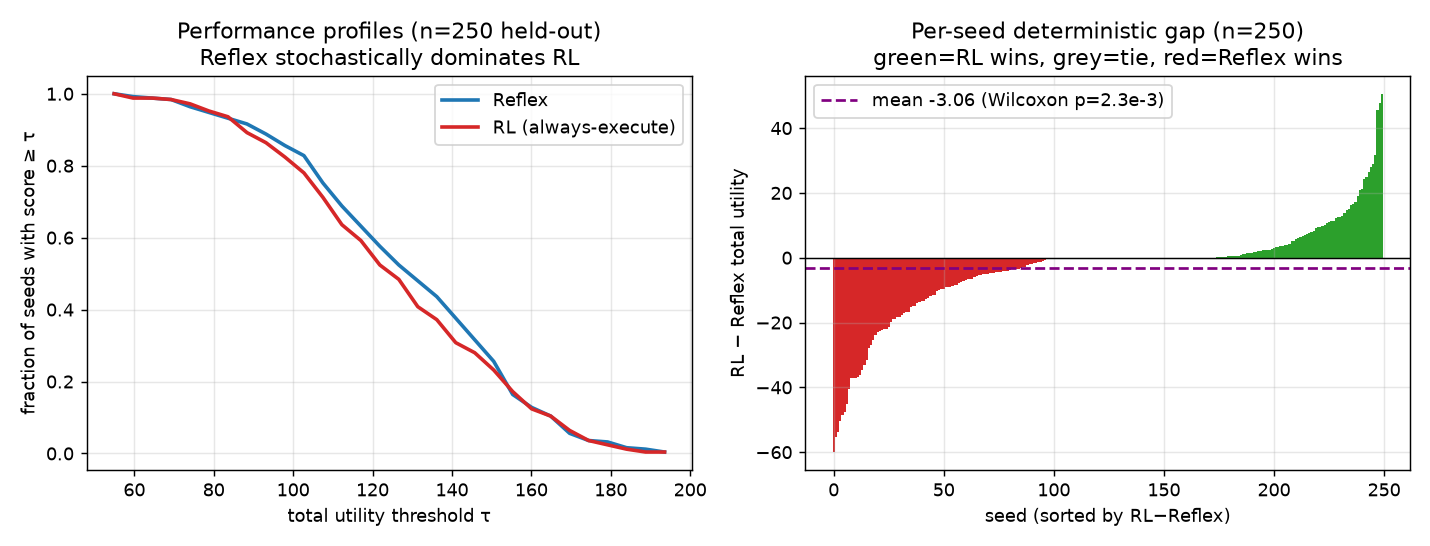
\includegraphics[width=\columnwidth]{fig_power_rliable.png}
\caption{Left: performance profiles on the $n=250$ pool --- Reflex (blue)
stochastically dominates the learned always-execute policy (red). Right: per-seed
$\text{Learned}-\text{Reflex}$ utility (green = learner wins, grey = exact tie,
red = Reflex wins); mean $-3.06$, $p=2.3\times10^{-3}$.}
\label{fig:power}
\end{figure}

\subsection{The Taxonomy: When Always-Execute Appears, and Why}
\label{sec:taxonomy}

We now vary the environment so that a non-execute action provably pays, and ask
two questions of each environment: does the lever exist (Table~\ref{tab:levers}),
and do the two learners find it (Table~\ref{tab:taxonomy}, Figure~\ref{fig:tax})?

\begin{table}[t]
\centering
\caption{Lever check: a hand-crafted reference policy vs.\ always-execute on each
environment ($50$ seeds, true metric). A positive significant $\Delta$ means a
non-execute action pays.}
\label{tab:levers}
\small
\setlength{\tabcolsep}{4pt}
\begin{tabularx}{\columnwidth}{@{}Yccc@{}}
\toprule
\textbf{Environment} & \textbf{always-exec} & \textbf{reference} & \textbf{$\Delta$ ($p$)} \\
\midrule
\env{benign}     & $111.5$ & $114.3$ & $+2.8\ (0.06)$ \\
\env{tight}      & $82.8$  & $89.1$  & $+6.2\ (0.03)$ \\
\env{heavytail}  & $451.6$ & $470.0$ & $+18.5\ (0.03)$ \\
\env{cascade}    & $21.0$  & $34.1$  & $+13.1\ (0.01)$ \\
\bottomrule
\end{tabularx}
\end{table}

\begin{table*}[t]
\centering
\caption{The taxonomy. Utility on the $50$-seed held-out pool (true metric);
$\Delta$ is vs.\ always-execute. ``A-E util'' is the always-execute utility;
each learner column gives $\Delta$ for three initialisation seeds.
\textbf{Bold} marks a significant escape from always-execute ($p<0.05$).}
\label{tab:taxonomy}
\small
\setlength{\tabcolsep}{4pt}
\begin{tabularx}{\textwidth}{@{}l c c
   >{\raggedright\arraybackslash}p{2.7cm}
   >{\raggedright\arraybackslash}p{2.7cm} Y@{}}
\toprule
\textbf{Environment} & \textbf{A-E util} & \textbf{ref.\ $\Delta$}
 & \textbf{REINFORCE $\Delta$ (3 seeds)} & \textbf{PPO $\Delta$ (3 seeds)} & \textbf{Determinant} \\
\midrule
\env{benign} (no lever)
 & $111.5$ & $+2.8$
 & --- (trivial by constr.)
 & $+0.8$ to $+1.5$; \newline $\approx\!100\%$ exec
 & \textbf{Environment}: optimum trivial; PPO correctly does not scale \\[3pt]
\env{tight} (scale, $+6$)
 & $82.8$ & $+6.2$
 & $+0.0$ (all 3, stuck)
 & $\mathbf{+21}$ to $\mathbf{+28}$ \newline (3/3, $p{<}10^{-7}$)
 & \textbf{Optimiser}: REINFORCE too weak; PPO escapes $3/3$ \\[3pt]
\env{heavytail} (scale, $+18$)
 & $451.6$ & $+18.5$
 & $+0.0$ (all 3, stuck)
 & $\mathbf{+14}$ to $\mathbf{+15}$ \newline (2/3; seed 7: $-1.3$)
 & \textbf{Optimiser}: PPO escapes $2/3$; whale variance defeats the 3rd \\[3pt]
\env{cascade}, fixed reward (caution, $+120$)
 & $21.0$ & $+13.1$
 & $\mathbf{+120}$ \newline ($51\%\!\to\!5\%$ fail)
 & $\mathbf{+98}$ to $\mathbf{+122}$
 & Adequate reward $+$ lever: both learn caution \\[3pt]
\env{cascade-broken} (A1 bug)
 & $21.0$ & $+13.1$
 & $+0.0$ (reckless, $51\%$ fail)
 & $+18.0$ (partial)
 & \textbf{Reward bug}: removes the direct failure signal \\
\bottomrule
\end{tabularx}
\end{table*}

\begin{figure*}[t]
\centering
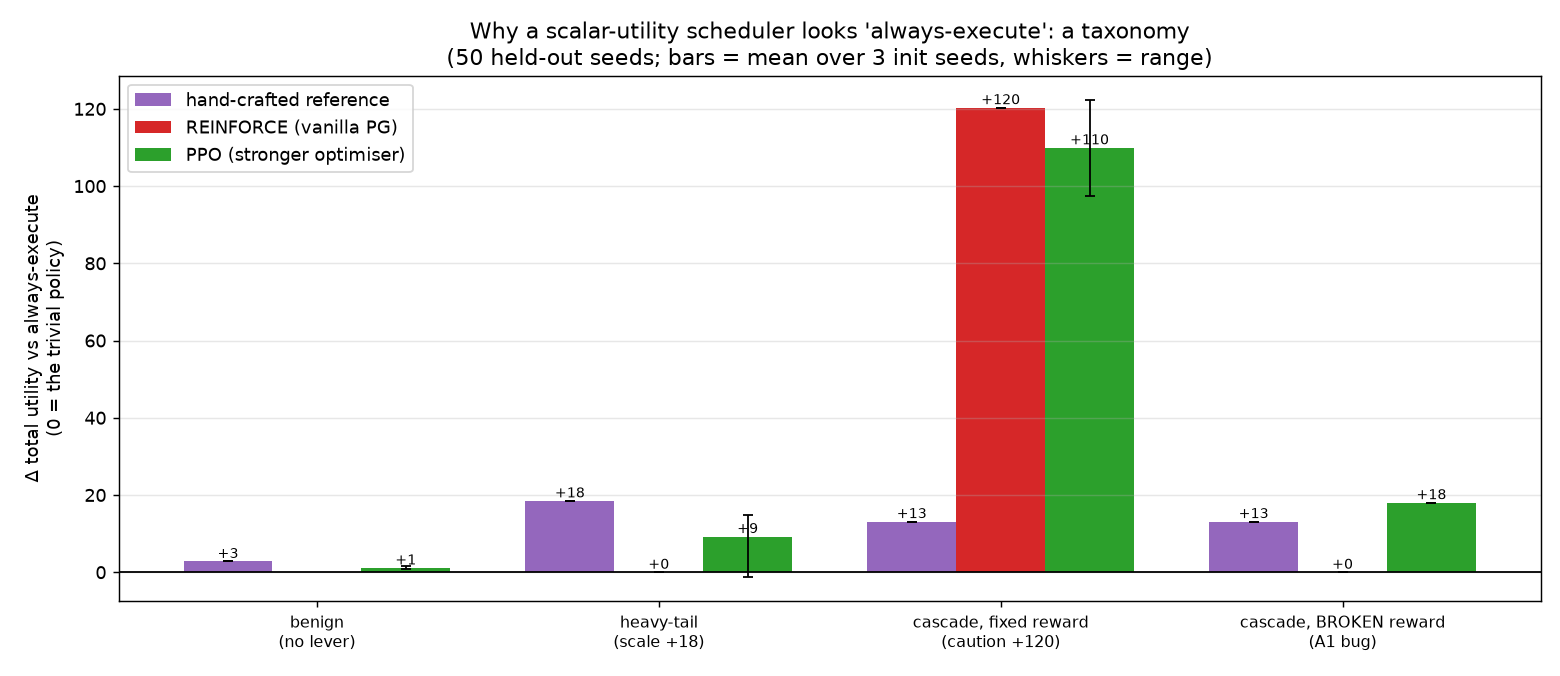
\includegraphics[width=0.92\textwidth]{fig_taxonomy.png}
\caption{Why a scalar-utility scheduler looks ``always-execute'': a taxonomy.
Bars are $\Delta$ utility vs.\ always-execute (the $0$ line is the trivial
policy), mean over three initialisation seeds, whiskers the range, on $50$
held-out seeds. REINFORCE (red) sits at $\approx 0$ wherever the lever is a modest
scaling improvement (\env{tight}, \env{heavytail}) and rises only at the enormous
caution lever (\env{cascade}); PPO (green) rises wherever a lever exists and the
reward is correct, and correctly stays near $0$ on the benign environment.}
\label{fig:tax}
\end{figure*}

Four findings follow.

\paragraph{(i) Benign: every competent agent stays trivial.} On the benign
environment, PPO converges to $\approx\!100\%$ execute, $+1.0$ utility over
always-execute --- statistically above zero but operationally identical to the
trivial policy, and well below the $+6$ to $+28$ it achieves where scaling pays.
Crucially, PPO \emph{declines} to scale here even though it scales aggressively
elsewhere: it is not biased toward any action, it adapts to the environment.

\paragraph{(ii) Optimiser, not reward.} On \env{tight} (scaling worth $+6.2$,
$p=0.03$), REINFORCE is stuck at $100\%$ execute on all three seeds ($\Delta=0.0$),
while PPO learns to scale on all three and beats always-execute by $+21$ to $+28$
utility ($p<10^{-7}$), lifting completion from $0.42$ to $0.58$. On
\env{heavytail} (scaling worth $+18.5$, with whales worth $50$ each), REINFORCE is
again stuck on all three seeds, and PPO escapes on two of three ($+14$ to $+15$,
$p<10^{-5}$); the third is defeated by the high return variance the whales induce.
We confirmed this is a genuine optimisation failure and not a discount artifact:
on \env{tight} the scaling reference beats always-execute on the discounted
training return as well ($+2.06$, $p=0.01$), so REINFORCE's own objective prefers
scaling, yet it does not find it. Under the \emph{identical} reward and
environment, a stronger optimiser removes the attractor.

\paragraph{(iii) The reward bug is material.} On \env{cascade}, where overload
triggers cascading failures, the corrected reward turns REINFORCE into a careful
policy: it learns to scale up to hold load below the failure threshold, cutting
the failure rate from $51\%$ to $5\%$ and lifting utility by $+120$
($p=1.8\times10^{-15}$). With the original (buggy) reward
(\env{cascade-broken}), the same REINFORCE stays byte-identical to reckless
always-execute ($51\%$ failure), and even PPO recovers only $+18$ --- from the
\emph{indirect} value signal (failed jobs forfeit value), not from the missing
failure penalty. The reward fix matters most for the weaker optimiser ($0\to+120$)
and substantially for the stronger one ($+18\to+122$).

\paragraph{(iv) REINFORCE's threshold.} REINFORCE escapes always-execute only when
the lever is enormous (\env{cascade}, $+120$); it fails the modest scaling levers
($+6$, $+18$) on all six seeds. PPO escapes whenever a lever exists and the reward
is correct ($5/6$ scaling seeds), and abstains correctly where none exists. The
determinant of ``always-execute'' is the environment, the optimiser, or a reward
bug --- in no cell is it the reward's linear shape.

\subsection{Behavioural Summary}
\label{sec:behaviour}

Inspection of the learned policies confirms the table. The benign and stuck
policies emit \term{Execute} on $100\%$ of steps. The escaping PPO policies on
\env{tight}/\env{heavytail} emit \term{Scale\_Up} on $7$--$11\%$ of steps ---
concentrated in capacity-blocked states --- and otherwise execute. The
caution-learning policies on \env{cascade} emit \term{Scale\_Up} to keep CPU load
below the cascade threshold, a single emergent rule that simultaneously raises
throughput and avoids failures. No policy uses \term{Reprioritize\_Queue} or
\term{Pause\_LowPriority\_Job}, consistent with those actions being net-negative
in every environment we tested.

% =============================================================================
\section{Discussion}
\label{sec:discussion}

\paragraph{The retracted claim.} The earlier framing --- that the reward's shape,
not the algorithm and not the observation, determines the always-execute
attractor --- is false in every cell of Table~\ref{tab:taxonomy}. The invariances
that motivated it (to reward weights, observation dimension, and seed) are real
but uninformative, because they leave fixed the two factors that actually move the
outcome: the environment and the optimiser. The honest contribution is the
taxonomy: a scalar-utility scheduler looks trivial when the environment has a
trivial optimum, when the optimiser is too weak to find a real but modest
improvement, or when the reward is mis-specified.

\paragraph{Why a CMDP is not ``the corrective.''} An earlier draft proposed
reformulating the scalarised utility as a constrained MDP with learned dual
multipliers as ``the corrective the mathematics implies.''
Table~\ref{tab:taxonomy} shows this is mistargeted. On the benign environment a
CMDP cannot manufacture a non-trivial optimum, because none exists --- there is no
caution lever for a constraint to bind on. On \env{tight}, \env{heavytail}, and
\env{cascade}, the lever is real, and the corrective that actually works is a
stronger \emph{optimiser} (PPO) or the \emph{corrected scalar reward} --- neither
of which is a CMDP. The CMDP machinery may still be valuable for guaranteeing hard
cost or failure budgets, but it is not the explanation for, or the fix to, the
trivial attractor.

\paragraph{Implications for practice.} Three lessons generalise beyond this
simulator. First, before concluding that a scalar reward is to blame for a trivial
learned policy, verify that the environment actually contains states where a
non-trivial action pays; if it does not, the learner is correct. Second, a
deep-RL ``failure to beat a simple baseline'' should be tested against a stronger
optimiser before it is attributed to the objective: a modest, delayed improvement
can be invisible to a high-variance estimator (REINFORCE) and obvious to a
low-variance one (PPO). Third, verify the reward identity --- that the cumulative
per-step reward equals the reported metric --- as a unit test; a telescoping
defect on one term can silently delete an entire objective.

\paragraph{Reframing the original ``negative result.''} What survives is more
useful than the original claim. We document a clean case in which an apparent
``RL collapses to a trivial policy'' result decomposes into a correct learner on a
trivial environment, a weak optimiser on a non-trivial one, and a reward bug ---
and in which a competent learner, given a lever and a correct reward, adapts. That
a careful, minimally confounded study of a scalar-utility scheduler can be fooled
in three distinct ways is a more instructive message for the systems-RL community
than a single ``reward-shape failure mode.''

% =============================================================================
\section{Threats to Validity}
\label{sec:threats}

\paragraph{Simulator fidelity.} The environment is a discrete-time single-cluster
abstraction; it omits JVM warmup, executor motion, network and disk I/O, and
straggler effects present in production Spark/Kubernetes systems. The taxonomy is
a statement about the gradient landscape of a scalar utility under controlled
environment edits; whether the specific operational consequences transfer to a
production system is a real-system validation we do not claim.

\paragraph{Optimiser scope.} We test REINFORCE and PPO. The claim ``a stronger
optimiser escapes the attractor'' is demonstrated for PPO; we do not claim every
algorithm escapes, and PPO itself fails one of three \env{heavytail} seeds. The
honest statement is that the attractor is \emph{not} algorithm-independent, which
is the opposite of the earlier draft's assertion.

\paragraph{Environment coverage.} The five environments are minimal edits chosen
to isolate single levers (scaling, caution, value heterogeneity). They are not a
random sample of production workloads; a heavy-tailed, capacity-exceeding,
arrival-driven workload would exercise more levers simultaneously and is the
natural next step.

\paragraph{Heavy-tail variance.} On \env{heavytail}, the whale-induced return
variance defeats PPO on one seed; this is a property of value-function credit
assignment under heavy-tailed rewards and suggests reward normalisation or
distributional critics as remedies, which we do not evaluate.

% =============================================================================
\section{Reproducibility}
\label{sec:repro}

All results trace to committed scripts and CSV artifacts. Each training and
evaluation run writes a resolved configuration, a manifest (commit hash, config
hash, seed list, library versions, wall-clock), and per-seed metrics. Seeds are
partitioned into disjoint pools enforced at configuration load, and every new
experiment's pool and prediction were registered before running. The diagnostics
(\S\ref{sec:methods}) --- the reward-identity check, the local-optimality probe,
the power/rliable analysis --- and the five environment configurations are
generated by committed scripts; the full taxonomy
(Table~\ref{tab:taxonomy}, Figure~\ref{fig:tax}) regenerates from a single
evaluation script and its CSV. The complete test suite ($140$ tests) passes on a
pinned environment. Code and artifacts are released
\cite{mohamed2026repo}.

% =============================================================================
\section{Conclusion}
\label{sec:conclusion}

A self-learning agent maximising a scalar utility for data-pipeline orchestration
converges to a trivial always-execute policy. The tempting explanation --- that
the reward's shape causes it --- is false. We replace it with a measured
taxonomy: always-execute appears because the environment's optimum is genuinely
trivial, because the optimiser (REINFORCE) cannot find a real but modest
improvement that a stronger optimiser (PPO) finds easily, or because a
reward-specification defect deletes the failure penalty. We further correct an
underpowered equivalence claim, showing the learned policy is significantly if
slightly worse than a trivial reflex baseline. A competent learner, given an
environment with a lever and a correctly specified reward, adapts --- scaling
where scaling pays, throttling where caution pays, and abstaining where neither
does. The lesson for systems reinforcement learning is to attribute a trivial
learned policy to the environment, the optimiser, or the reward identity ---
checked individually --- before attributing it to the shape of the objective.

\printbibliography

\end{document}
